\documentclass[12pt]{report}
\usepackage[utf8]{inputenc}
\usepackage[russian]{babel}
%\usepackage[14pt]{extsizes}
\usepackage{listings}
\usepackage{graphicx}
\usepackage{amsmath,amsfonts,amssymb,amsthm,mathtools} 
\usepackage{pgfplots}
\usepackage{filecontents}
\usepackage{indentfirst}
\usepackage{eucal}
\usepackage{enumitem}
\frenchspacing

\usepackage{indentfirst} % Красная строка


\usetikzlibrary{datavisualization}
\usetikzlibrary{datavisualization.formats.functions}

\usepackage{amsmath}




% Для листинга кода:
\lstset{ %
language=python,                 % выбор языка для подсветки
basicstyle=\small\sffamily, % размер и начертание шрифта для подсветки кода
numbers=left,               % где поставить нумерацию строк (слева\справа)
numberstyle=\tiny,           % размер шрифта для номеров строк
stepnumber=1,                   % размер шага между двумя номерами строк
numbersep=5pt,                % как далеко отстоят номера строк от подсвечиваемого кода
showspaces=false,            % показывать или нет пробелы специальными отступами
showstringspaces=false,      % показывать или нет пробелы в строках
showtabs=false,             % показывать или нет табуляцию в строках
frame=single,              % рисовать рамку вокруг кода
tabsize=2,                 % размер табуляции по умолчанию равен 2 пробелам
captionpos=t,              % позиция заголовка вверху [t] или внизу [b] 
breaklines=true,           % автоматически переносить строки (да\нет)
breakatwhitespace=false, % переносить строки только если есть пробел
escapeinside={\#*}{*)}   % если нужно добавить комментарии в коде
}

\usepackage[left=2cm,right=2cm, top=2cm,bottom=2cm,bindingoffset=0cm]{geometry}
% Для измененных титулов глав:
\usepackage{titlesec, blindtext, color} % подключаем нужные пакеты
\definecolor{gray75}{gray}{0.75} % определяем цвет
\newcommand{\hsp}{\hspace{20pt}} % длина линии в 20pt
% titleformat определяет стиль
\titleformat{\chapter}[hang]{\Huge\bfseries}{\thechapter\hsp\textcolor{gray75}{|}\hsp}{0pt}{\Huge\bfseries}


% plot
\usepackage{pgfplots}
\usepackage{filecontents}
\usetikzlibrary{datavisualization}
\usetikzlibrary{datavisualization.formats.functions}

\begin{document}
\thispagestyle{empty}
\begin{titlepage}
	\noindent \begin{minipage}{0.15\textwidth}
	
\includegraphics[width=\linewidth]{b_logo}
	\end{minipage}
	\noindent\begin{minipage}{0.9\textwidth}\centering
		\textbf{Министерство науки и высшего образования Российской Федерации}\\
		\textbf{Федеральное государственное бюджетное образовательное учреждение высшего образования}\\
		\textbf{~~~«Московский государственный технический университет имени Н.Э.~Баумана}\\
		\textbf{(национальный исследовательский университет)»}\\
		\textbf{(МГТУ им. Н.Э.~Баумана)}
	\end{minipage}
	
	\noindent\rule{18cm}{3pt}
	\newline\newline
	\noindent ФАКУЛЬТЕТ $\underline{\text{«Информатика и системы управления»}}$ \newline\newline
	\noindent КАФЕДРА $\underline{\text{«Программное обеспечение ЭВМ и информационные технологии»}}$\newline\newline\newline\newline\newline
	
	
	\begin{center}
		\noindent\begin{minipage}{1.3\textwidth}\centering
			\Large\textbf{  Отчет по лабораторной работе №1}\newline
			\textbf{по дисциплине "Анализ алгоритмов"}\newline\newline
		\end{minipage}
	\end{center}
	
	\noindent\textbf{Тема} $\underline{\text{Расстояние Левенштейна и Дамерау-Левенштейна}}$\newline\newline
	\noindent\textbf{Студент} $\underline{\text{Андрич К. }}$\newline\newline
	\noindent\textbf{Группа} $\underline{\text{ИУ7И-56Б}}$\newline\newline
	\noindent\textbf{Оценка (баллы)} $\underline{\text{~~~~~~~~~~~~~~~~~~~~~~~~~~~}}$\newline\newline
	\noindent\textbf{Преподаватели} $\underline{\text{Волкова Л.Л.}}$\newline\newline\newline
	
	\begin{center}
		\vfill
		Москва~---~\the\year
		~г.
	\end{center}
\end{titlepage}


\tableofcontents

\newpage
\chapter*{Введение}
\addcontentsline{toc}{chapter}{Введение}
\textbf{Расстояние Левенштейна} - минимальное количество операций вставки одного символа, удаления одного символа и замены одного символа на другой, необходимых для превращения одной строки в другую.
\newline

Расстояние Левенштейна применяется в теории информации и компьютерной лингвистики для:

\begin{itemize}
	\item исправления ошибок в слове
	\item сравнения текстовых файлов утилитой diff
	\item в биоинформатике для сравнения генов, хромосом и белков
\end{itemize}

Целью работы является изучение метода динамического программирования на материале алгоритмов нахождения расстояния Левенштейна и Дамерау-Левенштейна и оценка их реализаций.
\newline

Задачи лабораторной работы:
\begin{enumerate}
  	\item Изучение алгоритмов Левенштейна и Дамерау-Левенштейна;
	\item Получение практических навыков реализации указанных алгоритмов: матричные и рекурсивные версии; 
	\item Сравнительный анализ реализаций выбранного алгоритма определения расстояния между строками по затрачиваемым ресурсам; 
	\item Экспериментальное подтверждение различий во временнóй эффективности 
	реализаций выбранного алгоритма; 
	\item Описание и обоснование полученных результатов в отчете о выполненной лабораторной
работе, выполненного как расчётно-пояснительная записка к работе. 
\end{enumerate}

\chapter{Аналитическая часть}

Расстояние Левенштейна \cite{Levenshtein} между двумя строками — это минимальное количество операций вставки, удаления и замены, необходимых для превращения одной строки в другую.


При преобразовании одного слова в другое можно использовать следующие
операции:

\begin{itemize}
	\item D (от англ. delete) - удаление.
	\item I (от англ. insert) - вставка.
	\item R (от англ. replace) - замена.
\end{itemize}

Будем считать стоимость каждой вышеизложенной операции - 1.
Введем понятие совпадения - M (от англ. match). Его стоимость будет равна
0.

\section{Расстояниe Левенштейна}

Имеем две строки S1 и S2, длинной M и N соответственно. Расстояние Левенштейна рассчитывается по рекуррентной формуле:
\begin{equation}
	D(S_1[1...i],S_2[1...j]) = \left\{ \begin{array}{ll}
		$j, если i == 0$\\
		$i, если j == 0$\\
		min(\\
		D(S_1[1...i],S_2[1...j-1]) + 1,\\
		D(S_1[1...i-1], S_2[1...j]) + 1, & $j>0, i>0$\\
		D(S_1[1...i-1], S_2[1...j-1]) + \\
		\left[ 
		\begin{array}{c} 
			$0, если $S_1$[i] == $S_2$[j]$\\
			$1, иначе$
		\end{array}
		\right.\\
		)
	\end{array} \right.
\end{equation}


\section{Расстояние Дамерау-Левенштейна}

Как было написано выше, в расстоянии Дамерау-Левенштейна задействует еще одну редакторскую операцию - транспозицию T (\textit{от англ. transposition}). 
Расстояние Дамерау-Левенштейна рассчитывается по рекуррентной формуле:

\begin{equation}
	D(S_1[1...i],S_2[1...j]) = \left\{ \begin{array}{ll}
		$j, если i == 0$\\
		$i, если j == 0$\\
		min(\\
		D(S_1[1...i],S_2[1...j-1]) + 1,\\
		D(S_1[1...i-1], S_2[1...j]) + 1, & \textrm{$j>0, i>0$}\\
		D(S_1[1...i-1], S_2[1...j-1]) + \\
		\left[ 
		\begin{array}{c} 
			$0, если $S_1$[i] == $S_2$[j]$\\
			$1, иначе,$
		\end{array}
		\right.\\
		\left[ 
		\begin{array}{c} 
			D(S_1[1...i-2],S_2[1...j-2]) + 1, $ если $ $i, j>1, $a_i=b_{j-1}, b_j=a_{i-1}\\
			\infty $ , иначе )$ 
		\end{array}
		\right.\\
	\end{array} \right.
\end{equation}

\section{Вывод}
	В данном разделе были рассмотрены алгоритмы нахождения расстояния Левенштейна и Дамерау-Левенштейна, который является модификаций первого, учитывающего возможность перестановки соседних символов. Aлгоритмы могут быть реализованы рекурсивно или матрично.
	
\clearpage

\chapter{Конструкторская часть}

\section{Схемы алгоритмов}
В данной части будут рассмотрены схемы алгоритмов нахождения расстояние Левештейна и Дамерау - Левенштейна. На рисунках 2.1 - 2.4 представлены рассматриваемые алгоритмы.

\begin{figure}[h]
	\centering
	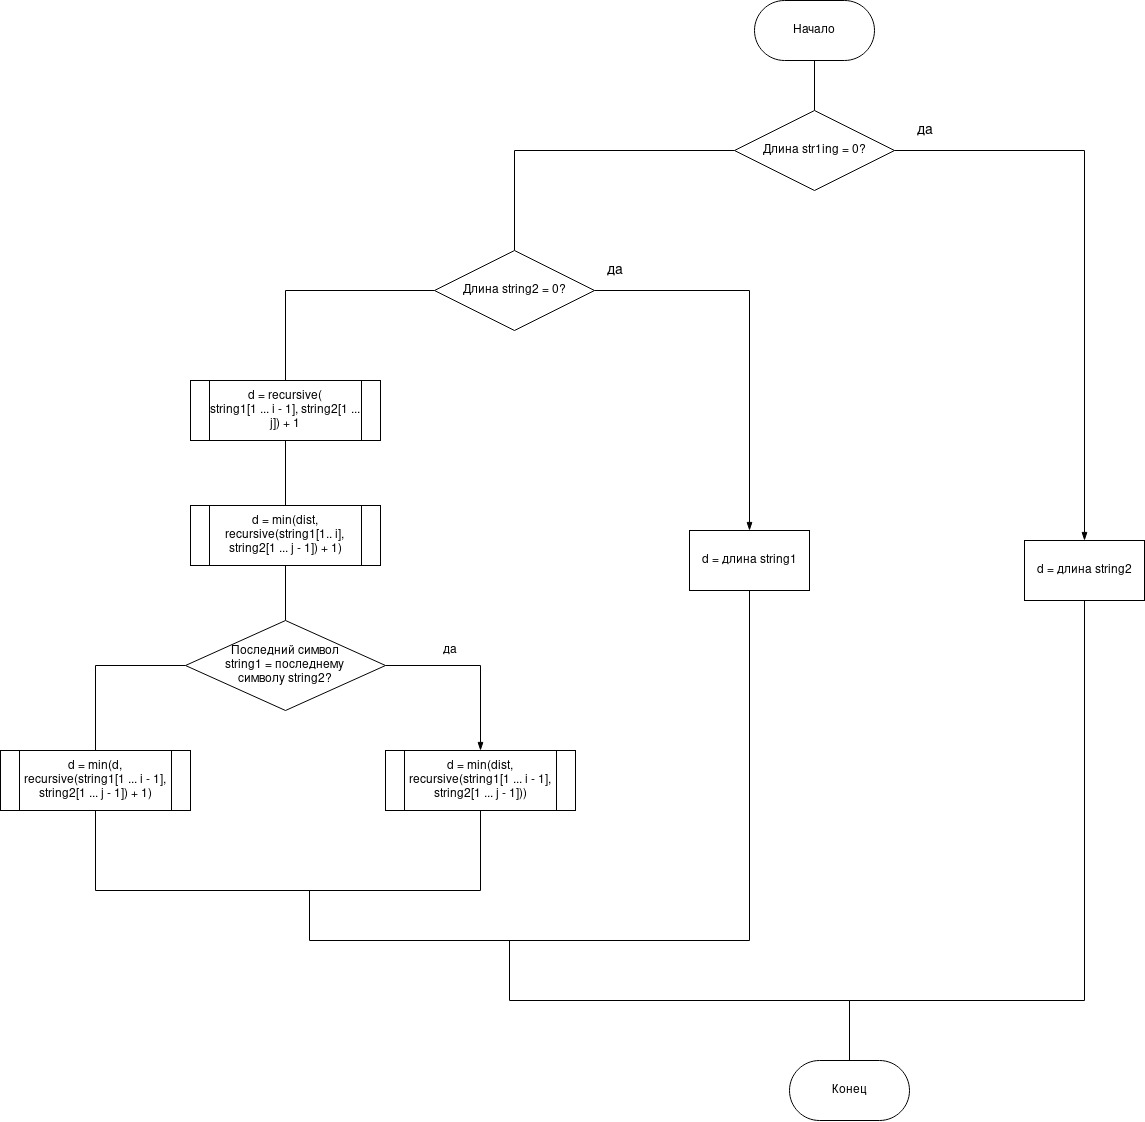
\includegraphics[width=0.75\linewidth]{rec.jpg}
	\caption{Схема рекурсивного алгоритма нахождения расстояния Левенштейна}
	\label{fig:mpr}
\end{figure}

\newpage

\begin{figure}[h]
	\centering
	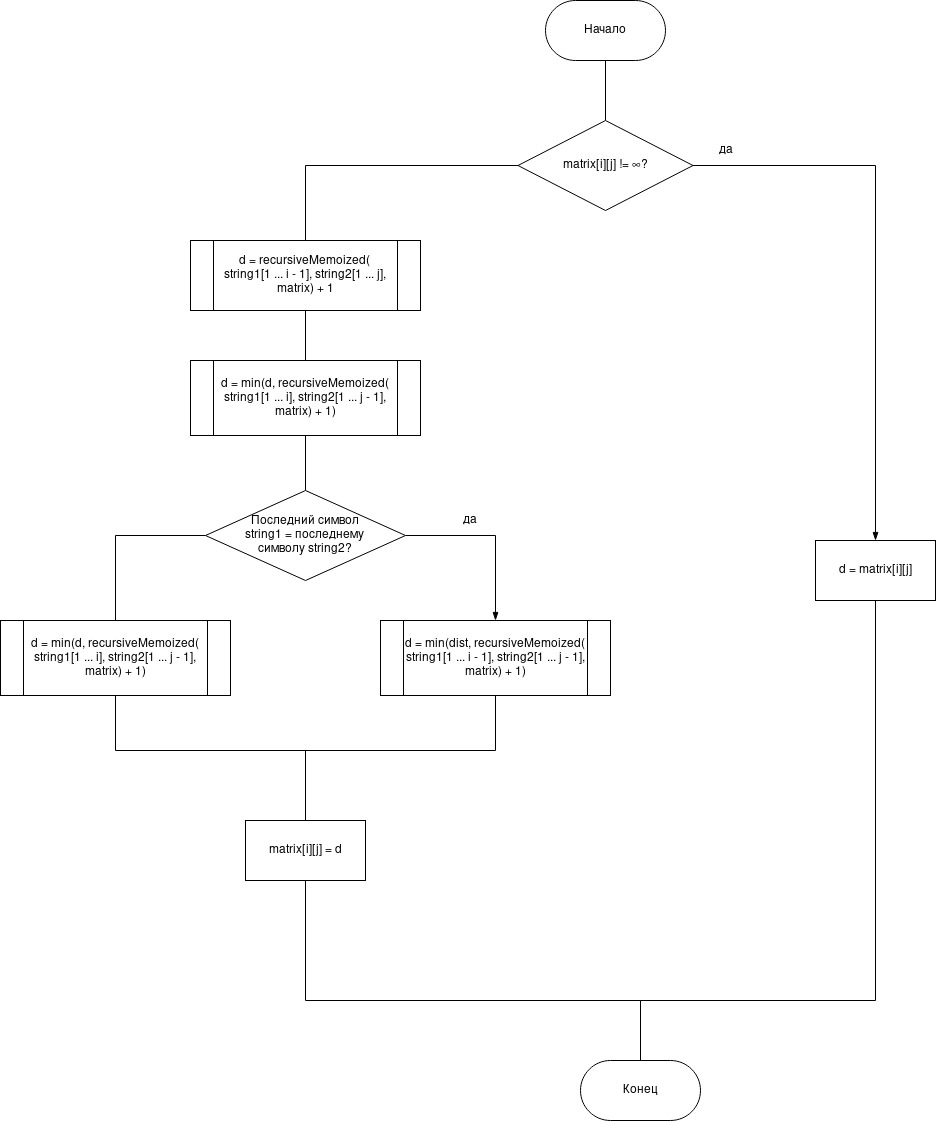
\includegraphics[scale=0.4]{mem.jpg}
	\caption{Схема рекурсивного алгоритма Левенштейна с кэшем}
	\label{fig:mpr}
\end{figure}

\newpage

\begin{figure}[h]
	\centering
	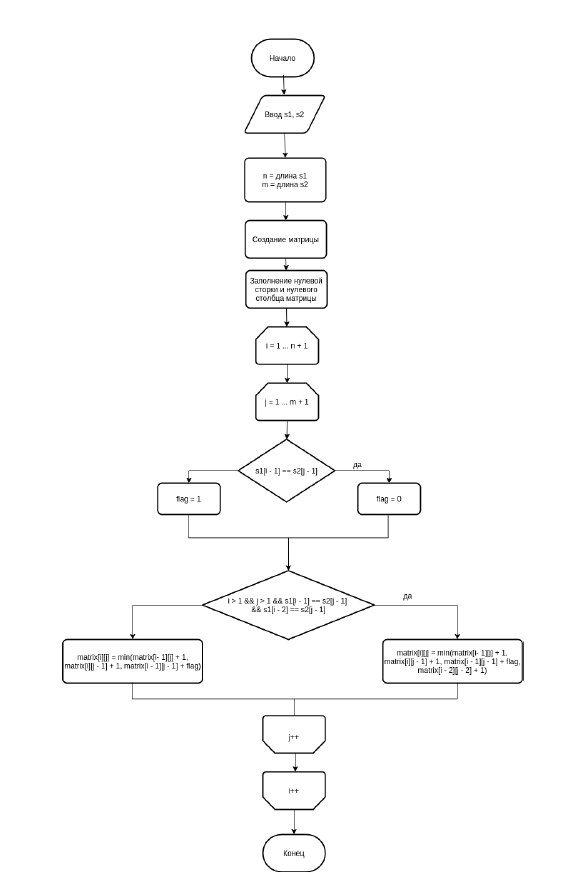
\includegraphics[scale=1]{dlmtrx.jpg}
	\caption{Схема алгоритма поиска расстояния Дамерау–Левенштейна
		с помощью матрицы(без рекурсии)}
	\label{fig:mpr}
\end{figure}

\newpage

\section{Вывод}
	На основе теоретических данных, полученные в аналитическом разделе были построены схемы иследуеммых  алгоритмов.

\chapter{Технологическая часть}

\section{Выбор ЯП}
В данной лабораторной работе использовался язык программирования - python. Данный выбор обусловлен тем, что этот язык наиболее удобен для работы со строками, а также тем, что в нём присутсвует функция для измерения процессорного времени.
В качестве среды разработки я использовала Visual Studio Code, так как считаю его достаточно удобным.

\section{Требование к ПО}
\textbf{Требования к вводу:}
\begin{enumerate}
	\item На вход подаются две строки в любой раскладке (в том числе и пустые);
	\item ПО должно выводить полученное расстояние;
	\item ПО должно выводить потраченное время;
\end{enumerate}

\section{Реализация алгоритмов}

В листингах 3.1 - 3.4 приведена реализация алгоритмов нахождения расстояния Левенштейна и Дамерау-Левенштейна.

\begin{lstlisting}[label=some-code,caption=Функция нахождения расстояния Левенштейна рекурсивно,language=Python]
def lev_recursion(str1, str2, len1, len2):
	if (len1 == len2) and len1 == 0:
		return 0
	elif len1 == 0:
		return len2
	elif len2 == 0:
		return len1
	else:
	flag = bool(not (str1[len1 - 1] == str2[len2 - 1]))
	return min(min(lev_recursion(str1, str2, len1 - 1, len2) + 1,
					lev_recursion(str1, str2, len1, len2 - 1) + 1),
					lev_recursion(str1, str2, len1 - 1, len2 - 1) + flag)
\end{lstlisting}

\begin{lstlisting}[label=some-code,caption=Функция нахождения расстояние Левенштейна рекурсивно с помощью кэша,language=Python]
def lev_cache(str1, str2, len1, len2, mtx):
	if not mtx[len1][len2] == 0:
		return mtx[len1][len2]
	elif (len1 == len2) and (len1 == 0):
		mtx[len1][len2] = 0
	elif len1 == 0:
		mtx[len1][len2] = len2
	elif len2 == 0:
		mtx[len1][len2] = len1
	else:
		flag = bool(not(str1[len1 - 1] == str2[len2 - 1]))
		mtx[len1][len2] = min(min(lev_cache(str1, str2, len1 - 1, len2, mtx) + 1,
								  lev_cache(str1, str2, len1, len2 - 1, mtx) + 1),
								  lev_cache(str1, str2,  len1 - 1, len2 - 1, mtx) + flag)
	return mtx[len1][len2]

def rec_lev_cache(str1, str2, len1, len2):
	mtx = [[0 for x in range(len2 + 1)] for y in range(len1 + 1)]
	return lev_cache(str1, str2, len1, len2, mtx)
\end{lstlisting}

\begin{lstlisting}[label=some-code,caption=Функция нахождения расстояния Дамерау-Левенштейна рекурсивно,language=Python]
	def lev_damau_recursion(str1, str2, len1, len2):
		if (len1 == len2) and len1 == 0:
			return 0
		elif len1 == 0:
			return len2
		elif len2 == 0:
			return len1
		else:
			flag = bool(not(str1[len1 - 1] == str2[len2 - 1]))
			res = min(lev_damau_recursion(str1, str2, len1 - 1, len2) + 1,
					lev_damau_recursion(str1, str2, len1, len2 - 1) + 1,
					lev_damau_recursion(str1, str2, len1 - 1, len2 - 1) + flag)
			if (len1 >= 2 and len2 >= 2 and str1[len1 - 1] == str2[len2 - 2] and str1[len1 - 2] == str2[len2 - 1]):
				res = min(res, lev_damau_recursion(str1, str2, len1 - 2, len2 - 2) + 1)
			return res 
\end{lstlisting}

\newpage

\begin{lstlisting}[label=some-code,caption=Функция нахождения расстояния Дамерау-Левенштейна матрично,language=Python]
def lev_damau_matrix(str1, str2, len1, len2):
	mtx = [[0 for x in range(len2 + 1)] for y in range(len1 + 1)]
	for i in range(len2 + 1):
		mtx[0][i] = i
	for i in range(1, len1 + 1):
		mtx[i][0] = i
	for i in range(1, len1 + 1):
		for j in range(1, len2 + 1):
			add, delete, change = mtx[i - 1][j] + 1, mtx[i][j - 1] + 1, mtx[i - 1][j - 1]
			if str2[j - 1] != str1[i - 1]:
				change += 1
			mtx[i][j] = min(add, delete, change)
			if ((i > 1 and j > 1) and str1[i - 1] == str2[j - 2] and str1[i - 2] == str2[j - 1]):
				mtx[i][j] = min(mtx[i][j], mtx[i - 2][j - 2] + 1)
	return mtx[len1][len2]
\end{lstlisting}

\section{Тестовые данные}

В таблице 3.1 приведены тестовые данные, на которых было протестированно разработанное ПО. Как видно из этой таблицы, все тесты были успешно пройдены, что означает, что программа работает правильно.

\begin{table}[h]
	\begin{center}
		\caption{Таблица тестовых данных}
		""\newline
		\begin{tabular}{|c c c c c|} 
			\hline
			№ & Первая строка & Вторая строка & Ожидаемый результат & Полученный результат \\ [0.8ex] 
			\hline
			1 & color & colour & 1 1 1 1 & 1 1 1 1\\
			\hline
			2 & padding & touchpad & 8 8 8 8 & 8 8 8 8\\
			\hline
			3 & kaska & taksa & 3 3 2 2 & 3 3 2 2\\
			\hline
			4 & lover & moped & 3 3 3 3 & 3 3 3 3\\
			\hline
			5 & lolly & lolyl & 2 2 1 1  & 2 2 1 1\\
			\hline
			6 & qwerty & queue & 4 4 4 4 & 4 4 4 4\\
			\hline
			7 & мама & папа & 2 2 2 2 & 2 2 2 2\\
			\hline
			8 &  & pat & 3 3 3 3 & 3 3 3 3\\
			\hline
			9 & baby &  & 4 4 4 4 & 4 4 4 4\\
			\hline
			10 &  &  & 0 0 0 0 & 0 0 0 0\\
			\hline
		\end{tabular}
	\end{center}
\end{table}

\section{Вывод}
В данном разделе были разработаны исходные коды четырех алгоритмов: вычисления расстояния Левенштейна рекурсивно и рекурсивно с использованием кэша, а также вычисления расстояния Дамерау — Левенштейна рекурсивно и с помощю матрицы.

\chapter{Исследовательская часть}

\section{Пример работы}

Демонстрация работы программы приведена на рисунке 4.1.

\begin{figure}[h]
	\begin{center}
	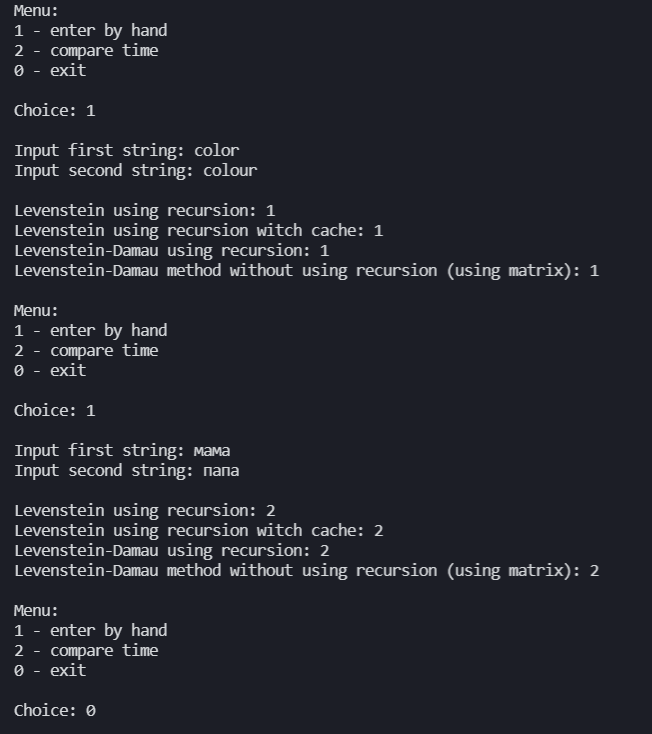
\includegraphics[scale=0.9]{example.png}
	 \caption{Работа алгоритмов нахождения расстояния Левенштейна и Дамерау -- Левенштейна.}
	\end{center}
\end{figure}

\section{Время выполнения алгоритмов}
Время выполнения алгоритмов замерялось с помощью функции process\_time модуля time в Python  \cite{process}. \newline

В таблице 4.1. представлены замеры времени работы для каждого из алгоритмов.

\begin{table} [h!]
	\caption{Таблица времени выполнения алгоритмов}
	\begin{center}
		\begin{tabular}{|c c c c c|} 
		 	\hline
			Длина строк & RecLev & RecLevCache & RecDam & MtxDam \\  
		 	\hline
		 	3 & 0.031250 & 0.031250 & 0.015625 & 0.015625\\
		 	\hline
		 	4 & 0.109375 & 0.031250 & 0.093750 & 0.015625 \\
		 	\hline
			5 & 0.484375 & 0.031250 & 0.531250 & 0.015625 \\
			\hline
			6 & 2.546875 & 0.046875 & 2.578125 & 0.031250 \\
			\hline
		\end{tabular}
	\end{center}
\end{table}

\begin{figure}[h!]
	\begin{center}
		\begin{tikzpicture}
			\begin{axis}[
				legend pos = north west,
				xlabel=длина строки,
				ylabel=секунды,
				minor tick num = 1,
				grid = both,
				major grid style = {lightgray},
				minor grid style = {lightgray!25},
				xtick distance = 50,
				width = 0.9\textwidth,
				height = 0.5\textwidth]
				
				\addplot[
				blue,
				semithick,
				mark = x,
				mark size = 3pt,
				thick,
				] file {LevRec.txt};
				
				\addplot[
				red,
				semithick,
				mark = *,
				] file {LevCache.txt};
				
				\legend{
					Рекурсивный алгоритм Левенштейна,
					Рекурсивный алгоритм Левенштейна с кэшем
				}
			\end{axis}
		\end{tikzpicture}
	\end{center}
	\caption{Сравнение рекурсивного алгоритма Левенштейна и рекурсивного с кэшем}
\end{figure}

\begin{figure}[h!]
	\begin{center}
		\begin{tikzpicture}
			\begin{axis}[
				legend pos = north west,
				xlabel=длина строки,
				ylabel=секунды,
				minor tick num = 1,
				grid = both,
				major grid style = {lightgray},
				minor grid style = {lightgray!25},
				xtick distance = 50,
				width = 0.9\textwidth,
				height = 0.5\textwidth]
				
				\addplot[
				blue,
				semithick,
				mark = x,
				mark size = 3pt,
				thick,
				] file {LevRec.txt};
				
				\addplot[
				red,
				semithick,
				mark = *,
				] file {DamLevRec.txt};
				
				\legend{
					Расстояние Левенштейна,
					Расстояние Дамерау -- Левенштейна
				}
			\end{axis}
		\end{tikzpicture}
	\end{center}
	\caption{Сравнение рекурсивных алгоритмов нахождения расстояния Левенштейна и Дамерау-Левенштейна}
\end{figure}

\newpage

\section{Использование памяти}

Алгоритмы нахождения расстояния Левенштейна и Дамерау — Левенштейна не отличаются друг от друга с точки зрения использования памяти.

Максимальная глубина стека вызовов при рекурсивной реализации равна сумме длин входящих строк. Поэтому, максимальный расход памяти равен: 

\begin{equation}
(\mathcal{S}(STR_1) + \mathcal{S}(STR_2)) \cdot (2 \cdot \mathcal{S}\mathrm{(string)} + 2 \cdot \mathcal{S}\mathrm{(integer)}),
\end{equation}

\noindent где $\mathcal{S}$ — оператор вычисления размера, $STR_1$, $STR_2$ — строки, $\mathrm{string}$ — строковый тип, 

\noindent $\mathrm{integer}$ — целочисленный тип.


\section{Вывод}

Обычная рекурсивная реализация алгоритма нахождения расстояния Левенштейна работает дольше реализации с кэшем, время работы этой реализации увеличивается в геометрической прогрессии. Рекурсивный метод при этом использует больше памяти.


\chapter*{Заключение}
\addcontentsline{toc}{chapter}{Заключение}

В ходе проделанной работы был изучен метод динамического программирования на материале реализации алгоритмов нахождения расстояния Левенштейна и Дамерау-Левенштейна. Также были изучены алгоритмы поиска расстояния Левенштейна и Дамерау-Левенштейна нахождения расстояния между строками и получены практические навыки раелизации указанных алгоритмов в матричной и рекурсивных версиях, а так же в версиях с мемоизацией.

Экспериментально было подтверждено различие во временной эффективности рекурсивной и нерекурсивной реализаций выбранного алгоритма определения расстояния между строками при помощи разработаного программного обеспечения на материале замеров процессорного времени выполнения реализации на варьирующихся длинах строк. 

Теоретически было рассчитано использование памяти в каждой из реализаций алгоритмов нахождения расстояния Левенштейна и Дамерау - Левенштейна.

\addcontentsline{toc}{chapter}{Список литератури}

\bibliographystyle{utf8gost705u}  % стилевой файл для оформления по ГОСТу

\bibliography{51-biblio}          % имя библиографической базы (bib-файла)

\begin{thebibliography}{9}
	\bibitem{Levenshtein} В. И. Левенштейн, Двоичные коды с исправлением выпадений, вставок и замещений символов. Доклады Академий Наук СССР, 1965. Т. 163 С. 845-848.
	
	\bibitem{atom} Intel Atom x7-E3950: технические характеристики и тесты [Электронный ресурс]. Режим доступа: https://technical.city/ru/cpu/Atom-x7-E3950. Дата обращения: 7.10.2021.
	
	\bibitem{process} Функция process\_time() модуля time в Python [Электронный ресурс]. Режим доступа: https://docs-python.ru/standart-library/modul-time-python/funktsija-process-time-modulja-time/. Дата обращения: 5.10.2021.
\end{thebibliography}

\end{document}
